%%%%%%%%%%%%%%%%%%%%%%%%%%%%%%%%%%%%%%%%%%%%%%%%%%%%%%%%%%%%%%%%%%
%%%%%%%% ICML 2015 EXAMPLE LATEX SUBMISSION FILE %%%%%%%%%%%%%%%%%
%%%%%%%%%%%%%%%%%%%%%%%%%%%%%%%%%%%%%%%%%%%%%%%%%%%%%%%%%%%%%%%%%%

% Use the following line _only_ if you're still using LaTeX 2.09.
%\documentstyle[icml2015,epsf,natbib]{article}
% If you rely on Latex2e packages, like most moden people use this:
\documentclass{article}

% use Times
\usepackage{times}
% For figures
\usepackage{graphicx} % more modern
%\usepackage{epsfig} % less modern
\usepackage{subfigure} 


% For citations
\usepackage{natbib}

% For algorithms
\usepackage{algorithm}
\usepackage{algorithmic}
\usepackage{amsmath}
\usepackage{amssymb}
\usepackage{todonotes}
\usepackage[nomarkers, nolists]{endfloat}
\renewcommand{\efloatseparator}{\mbox{}}

% As of 2011, we use the hyperref package to produce hyperlinks in the
% resulting PDF.  If this breaks your system, please commend out the
% following usepackage line and replace \usepackage{icml2015} with
% \usepackage[nohyperref]{icml2015} above.
\usepackage{hyperref}

% Packages hyperref and algorithmic misbehave sometimes.  We can fix
% this with the following command.
\newcommand{\theHalgorithm}{\arabic{algorithm}}
\def\code#1{\texttt{#1}}

% Employ the following version of the ``usepackage'' statement for
% submitting the draft version of the paper for review.  This will set
% the note in the first column to ``Under review.  Do not distribute.''
% \usepackage{icml2015} 

% Employ this version of the ``usepackage'' statement after the paper has
% been accepted, when creating the final version.  This will set the
% note in the first column to ``Proceedings of the...''
\usepackage[accepted]{icml2015}

\usepackage{enumitem}
\usepackage{bbm}
\usepackage{amsmath}
\usepackage{amsfonts}


\makeatletter
\def\BState{\State\hskip-\ALG@thistlm}
\makeatother




% The \icmltitle you define below is probably too long as a header.
% Therefore, a short form for the running title is supplied here:

% Saving space by deleting running title (does this actually save space?)
%\icmltitlerunning{Submission and Formatting Instructions for ICML 2015}

\begin{document} 

\twocolumn[

% Saving space by deleting title
%\icmltitle{Submission and Formatting Instructions for \\ 
%           International Conference on Machine Learning (ICML 2015)}

% It is OKAY to include author information, even for blind
% submissions: the style file will automatically remove it for you
% unless you've provided the [accepted] option to the icml2015
% package.
\icmlauthor{Lucas Manuelli}{manuelli@mit.edu}
\icmladdress{Massachusetts Institute of Technology}
\icmlauthor{Pete Florence}{peteflo@mit.edu}
\icmladdress{Massachusetts Institute of Technology}

% You may provide any keywords that you 
% find helpful for describing your paper; these are used to populate 
% the "keywords" metadata in the PDF but will not be shown in the document
\icmlkeywords{6.867, machine learning}

\vskip 0.3in
]

% Saving space by deleting abstract
%\begin{abstract} 
%The purpose of this document is to provide both the basic paper template and
%submission guidelines.
%\end{abstract} 

\section{Introduction}
In this project we evaluate the ability of several reinforcement learning methods to autonomously drive a car through a cluttered environment. We don't assume a map of the environment a priori but rather rely on our sensor (in this case a LIDAR) to make control decisions. A standard approach to solving this problem would require building up a map of the environment, possibly using an occupancy grid, and then planning a collision free path through this estimated map using a planner such as RRT*. On the other hand one notes that simple output feedback controllers, such as Braitenberg controllers, can be quite effective for obstacle avoidance tasks. Guided by this example we want to see how reinforcement learning performs in learning an output feedback controller.

Our initial goal was to implement a value-based learning method, and we were recommended to start with SARSA.  After some initial results with SARSA, we decided to also implement Q-learning, try function approximation, and also try policy search methods. 

In short, there were distinct advantages and items of concern found for the different approaches.    The value-function-based approaches benefit greatly from their Dynamic Programming formulation, but it is also their limitation, particularly due to the difficulties of discretization.  The policy-search-based approaches have some nice properties including that they are easy to ``seed'' with a favorable initialization, and do not need to be discretized, but do not benefit from Bellman's optimality principle.  In both cases, the ability of the reinforcement learning agents to improve their performance, even if not without ``hand-holding'' from us, is quite remarkable to watch.  That said, significant effort and tuning is required, and in the end, we were not able to satisfiably outperform intuitive hand-designed controllers.  The Dynamic Programming techniques had a ceiling of performance imposed by the discretization, and the policy search methods were not able to improve upon essentially-perfect hand-designed controllers.  Although this was the case for the study presented, it seems that in scenarios where intuition is less readily applied, and/or with more patient tuning of parameters, even better results may be obtained for the reinforcement learning controllers.

\section{Experiment Setup and Simulation Environment}

\subsection{Car Model}

For our car model we consider a simplified Dubin's car model. The location of the vehicle is described by $(x,y,\theta)$, where $(x,y)$ denote Cartesian position and $\theta$ denotes the orientation. For our purposes we suppose that we can control the derivative of the orientation, namely our control is $u = \dot{\theta}$. We also suppose a fixed speed $v$. Then the dynamics of the vehicle are given by
\todo{figure illustrating car + lidars}
%
%
\begin{align}
\dot{x} &= v \cos(\theta) \\ 
\dot{y} &= v \sin(\theta)\\ 
\dot{\theta} &= u
\end{align}
%
%
%

\subsection{Sensor Model}
For our sensor model we use a small array of point LIDARs. In particular, $N$ beams are spread evenly over the field of view $[\theta_{min},\theta_{max}]$.  All experiments shown use $N=20$ and $[\theta_{min}=-\pi,\theta_{max}=\pi]$.   Each laser has a maximum range of $d_{max}$. The $n^{th}$ laser then returns $x_n$, which is the distance to the first obstacle it encounters, or $d_{max}$ if no obstacle is detected. Then one laser measurement can be summarized as $X = (x_1,\ldots,x_N)$.

\subsection{Obstacle Environment}
Picking the right obstacle environment for our task required some trial-and-error.  Obstacles that were too thin along one direction were not a good choice, as they could hide in between the ``array of point LIDARs'' as the robot approached.  Thus circular obstacles were chosen, as they circumvented this problem.  Picking the right density of obstacles and obstacle size was another trial-and-error process.  A square border prevented the car from escaping.  A listing of approximate parameters for the obstacle environments used is provided below.  Generalizations across obstacle environments it outside the scope of this project.

\scalebox{0.7}{
  \begin{tabular}{l|c|c|l|c|c|c|c|c}
	\textbf{Car parameters}\\
	Car velocity, $v$ & 16 m/s \\ 
	Maximum turning rate, $u_{max}$ & 4 rad/s\\
	\\
	
	\textbf{Sensor parameters}\\
	Number of point LIDARS, N & 20 \\
	Maximum laser range, $d_{max}$ & 10 m \\
	Field of view $[\theta_{min},\theta_{max}]$ & $[-\pi, \pi]$ \\
	\\
	
	\textbf{Obstacle environment parameters}\\
	Area of square world & 250 $m^2$ \\
	Obstacle density & 0.18 / $m^2$ (45 obstacles in 250 $m^2$)\\
	Circular obstacle radius & 1.75 m \\
	
  \end{tabular}
}

\subsection{Simulation Environment}

Our software stack is integrated with a robotics visualization tool called Director \todo{director citation}. We use the Director code for visualization and raycasting. This is the only external code that we use in addition to standard Python modules. Our simulation environment is written in Python. We have a main class called \code{Simulator} which combines together several other modules, e.g. \code{Car}, \code{Sensor}, \code{World}, \code{Controller}, \code{Reward}, \code{Sarsa}, etc, to construct a working simulation class. All of this code was written by us for the project. As mentioned before, the only fundamental pieces of code that we didn't write were the visualization tools and the raycasting method which we use for computing our sensor model. One nice feature of the Director application is that it uses Visualization Toolkit as the underlying graphics engine, and thus our raycast calls are actually in C++ and thus very efficient. We use a timestep of $dt = 0.05$ in all our experiments, and \code{spicy.integrate} is used to for integrating forward the dynamics.

\subsection{Braitenberg (Hand-Designed) Controller}
\label{default_controller}
As a baseline against which to compare our learned controllers, we used a simple hand-designed controller inspired by the controllers of Valentino Braitenberg.  The most basic controller we tried simply counts the number of non-max sensor returns on the left ($n_{left} = \sum_i^{N/2} \mathbbm{1}[x_i < d_{max}]$) and compares with the number of non-max sensor returns on the right ($n_{right} = \sum_{i=N/2+1}^N \mathbbm{1}[x_i < d_{max}]$), and then selects the action to turn towards the direction $min(n_{left}, n_{right})$.  If no obstacles are seen ($n_{left} = n_{right} = 0$), then the controller selects to go straight.  Thus the action space for this simple controller is $A = \{-u_{max}, 0, u_{max} \}$.  This controller actually works surprisingly well.

The best Braitenberg-style controller we used is a slight improvement on the above version, but actually takes into the account the distances measured.  This controller uses the squared inverse of each of the sensor measurements as its features: $\phi_{B} (x_i) = \frac{1}{x_i^2}$.  The sum of these features is then computed for the left and right, and again the action is selected to turn towards the direction $min(n_{left}, n_{right})$.  An algorithm description is provided (Algorithm \ref{alg:bsic}).
%
\begin{algorithm}[]
   \caption{Braitenberg Squared Inverse Controller (BSIC)}
   \label{alg:bsic}
\begin{algorithmic}
   \STATE {\bfseries Input:} sensor data $x_i$, size $N$
   \STATE {\bfseries Output:} u from $\mathcal{A} =  \{-u_{max}, 0, u_{max}\}$
   \STATE Initialize $n_{left}$, $n_{right} = 0$
   \FOR{$i=1$  {\bfseries to} $N/2$}
   \STATE $n_{left} = n_{left} + 1/(x_i)^2$
   \ENDFOR
   \FOR{$i=N/2 + 1$  {\bfseries to} $N$}
   \STATE $n_{right} = n_{right} + 1/(x_i)^2$
   \ENDFOR
   \IF {$n_{left} > n_{right}$}
   \STATE $u = -u_{max}$ (TURN LEFT)
   \ELSE 
   \IF {$n_{left} < n_{right}$}
   \STATE $u = u_{max}$ (TURN RIGHT)
   \ELSE 
   \STATE $u=0$ (GO STRAIGHT)
   \ENDIF
   \ENDIF

\end{algorithmic}
\end{algorithm}



\section{Dynamic Programming: SARSA and Q-Learning}
Two of the most popular methods in reinforcement learning are SARSA and Q-Learning. These methods both aim to find the optimal policy of a dynamic programming problem. Thus the first step is to reformulate our problem as a dynamic programming problem. 

\subsection{Dynamic Programming Formulation}
To formulate our problem as a dynamic programming problem we need to define a ``state.'' Let $S_c = (x,y,\theta)$ be the state of the car, and let $X  = (x_1,\ldots,x_n)$ be the sensor state. In order to satisfy the Markov property, our reinforcement learning agent would also need to have access to the full state of the world, $S_{world}$, i.e. a complete description of each of the obstacles.  To make our problem similar to the limitations of a real car robot with just the described LIDAR sensor model, we only allow our reinforcement learning agent to access $X$, and so we consider $S = X$. Since this is not a state in the true sense of the word let us call it a reward state.  Next we need to define our action set. In principle our model has a continuous action set. However, for the purposes of SARSA and Q-Learning it is much easier to have a discrete action space. Thus we restrict ourselves to $a \in \{-u_{max},0,u_{max}\} = \mathcal{A}$, which correspond to left, straight, and right actions. Let $\theta_n$ be the angle of $n^{th}$ laser where $\theta_n = 0$ corresponds to straight ahead. Now we need to define the reward function. First define weights
%
%
\begin{equation}
w_n = r_0 + r_1 \cos(\theta_n)
\end{equation}
%
%
Also define
%
%
\begin{equation}
\phi(x_n) = \begin{cases}
\min(1/x_n, C_{max}) & x_n < d_{max}\\
0 & x_n = d_{max} 
\end{cases}
\end{equation}
%
%
Then $\phi$ has the effect of amplifying short distance measurements. Let $W = (w_1,\ldots,w_N)$, $\phi(X) = (\phi(x_1),\ldots,\phi(x_n))$. Then define the reward $R(S,a)$ as
%
%
\begin{equation}
R(S,a) = C_{action} |a| + \langle W, \phi(X) \rangle
\end{equation}
%
%
where $C_{action}$ is an action cost. Finally if the car is currently in collision with an obstacle, i.e. some laser $x_n$ is reading less than $d_{min}$ then we set $R(S,a) = C_{collision}$.

Now let us think about why this may be a reasonable reward function for our objective, which is obstacle avoidance. One should think of $r_0,r_1, C_{action}, C_{collision} < 0$ and $C_{max} > 0$. Then we see that the components of $\phi(X)$ increase as we get close to obstacles. And they increase as the inverse of the distance to the obstacle. Thus this is penalizing getting too close to obstacles. Now consider the weights $W$ show in Figure \ref{figures/raycastRewardWeights.png}
%
%
\begin{figure}
\centering
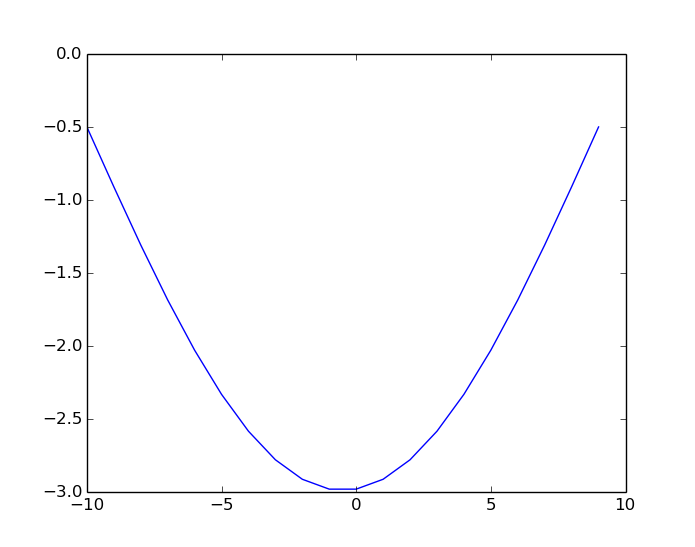
\includegraphics[scale=0.5]{figures/raycastRewardWeights.png}
\caption{$\lambda = 0.7$}
\label{figures/raycastRewardWeights.png}
\end{figure}
%
%
%
 This means that it's worse to have obstacles in front of you than off to the side. The action cost is to encourage the car to drive straight rather than spin around in circles. Finally since we are interested in obstacle avoidance we impose a large penalty if the car does crash into an obstacle.

The reason we have $\phi(X)$ and the weights $W$ is reward shaping. In reality all we care about is not crashing into obstacles, but it helps the algorithms to converge if the rewards ``guide'' them towards staying away from obstacles, e.g. if the reward is higher the further you are from the obstacles. 

Now that we have the reward function we can formulate our problem as a dynamic program. The problem is to find the policy $\pi:S \to \mathcal{A}$ to solve
%
%
\begin{equation}
\max_{\pi} E_{\pi} \left[ \sum_{t \geq 0} \gamma^t R(S_{t+1}, a_t) \right]
\end{equation}
%
%
The expectation is over the reward states that result from taking actions according to policy $\pi$. Here $\gamma \in (0,1)$ is a discount factor. In a standard dynamic programing framework the state $S_t$ would be Markov. That is, future states depend only on the current state and future actions. In our case however our reward state is non-Markov since the map of the world is not included as part of our state. 

\subsection{SARSA($\lambda$)}
\label{discrete_sarsa}
The difficulty with applying standard dynamic programming techniques to the current problem is that it is hard to write down the transition law $(S_t,a_t) \to S_{t+1}$ since this requires knowing how the sensor measurements will evolve. The SARSA technique allows us to circumvent this problem if we have access to runs/simulations of the true system. The Q-Values are defined as 
%
%
\begin{equation}
q_{\pi}(S,a) = E_{\pi} \left[ \sum_{k \geq 0} \gamma^k R(S_{t+k+1}, a_{t+k}) | S_t = s, A_t = a \right]
\end{equation}
%
%
Then if we knew the Q-values we could choose the best policy as 
%
\begin{equation}
\label{q-policy}
a = \arg \max_{a'} q_{\pi}(s,a) 
\end{equation}
%
The ultimate goal of SARSA($\lambda$) is to find the optimal policy $\pi^*$. Intuitively the approach is to estimate $q_{\pi}$ and then slowly improve the policy $\pi$ towards the optimal policy by using greedy policy selection based on the current q values. The algorithm is always estimating $q_{\pi}$ for the current policy $\pi$ and hence the q-values ultimately converge to $q_{\pi^*}$.

\begin{algorithm}[H]
   \caption{SARSA($\lambda$)}
   \label{alg:SARSA}
\begin{algorithmic}
   % \STATE {\bfseries Input:} sensor data $x_i$, size $N$
   % \STATE {\bfseries Output:} u from $\mathcal{A} =  \{-u_{max}, 0, u_{max}\}$
   \STATE Initialize $Q(S,a)$ arbitrarily for $S \in \mathcal{S}, a \in \mathcal{A}$
   \REPEAT
   \STATE{
   $Z(S,a) = 0$ for all $S \in \mathcal{S}, a \in \mathcal{A}$\\
   \FOR{each step of episode}
       \STATE Take action $A$, observe $R, S'$
       \STATE Choose action $A'$ from $S'$ using policy derived from $Q$ (e.g. $\epsilon$-greedy)
       \STATE $A* \leftarrow \arg \max_a Q(S',a)$ (if $A'$ ties for max then $A^* \leftarrow A'$)
       \STATE $\delta \leftarrow R + \gamma*Q(S',A') - Q(S,A)$
       \STATE $Z(S,A) \leftarrow Z(S,A) + 1$
       \FOR{ all $s \in \mathcal{S}, a \in \mathcal{A}$}
            \STATE $Q(s,a) \leftarrow Q(s,a) + \alpha \delta Z(s,a)$
            \IF{$A' = A^*$} 
                \STATE $Z(S,a) \leftarrow \gamma \lambda Z(s,a)$ 
            \ELSE{} 
                \STATE $Z(s,a) \leftarrow 0$
            \ENDIF
       \ENDFOR
       \STATE $S \leftarrow S', A \leftarrow A'$
   \ENDFOR}
   \UNTIL{end of episode}

\end{algorithmic}
\end{algorithm}




In order to apply SARSA in the form described above we need to discretize the state-action space. In section \ref{sarsa_function_approximation} we describe an approach that doesn't require discretizing the state. In order for the SARSA algorithm to be effective without drastically increasing the training time, we must keep the size of the discretization relatively small. With this in mind we chose a discretization based on bins. The discretization is governed by three parameters. $N_{inner}$, the number of inner bins, $N_{outer}$ the number of outer bins and $\beta_{cutoff}$, the cutoff distance (as a fraction of the maximum laser range) between inner and outer bins. A bin is defined by two angles $\theta_0, \theta_1$ and two distances $d_0, d_1$. Then this bin is occupied if any laser whose angle lies in $[\theta_0,\theta_1]$ returns a distance in $[d_0,d_1]$. For example suppose $N_{inner} = 5$ and $N = 20$. Then the lasers corresponding to this bin are $x_1,\ldots,x_4$. This bin would be occupied if $x_i \in [0, \beta_{cutoff}*d_max]$ for some $i \in \{1,\ldots,4\}$. If a bin is occupied then it is labeled with a $1$, if it is empty is is labeled with a zero. We have already discretized the action space into $\mathcal{A} = \{-4,0,4\}$. Thus the discretization of the state-action space lies in the space $\{0,1\}^{N_{inner} + N_{outer}} \times \mathcal{A}$. Hence the size of the discretization is $2^{N_{inner} + N_{outer}} \times |\mathcal{A}|$.



\subsubsection{Results}

There are many parameters that must be chosen in order to run the SARSA lambda algorithm. We discuss some of the most important here and give intuition on how we chose them. Then we will analyse how varying a few key parameters around our baseline setup affects performance. 

Two of the most important parameters are the number of bins $N_{inner}, N_{outer}$ in the discretization. You need enough bins that so that the state is informative enough to pass through relatively narrow gaps between obstacles. However adding more bins comes at the cost of increasing the size of the state space which can increase training time. In addition if a particular action-state pair is not visited sufficiently many times then that Q-value $Q(s,a)$ will not be a good approximation to the true Q-value, and hence control decisions taken based on that Q-value will not be optimal (and in fact will be quite poor usually). Through many experiments we found that $N_{inner} = 5, N_{outer} = 4$ provided good performance while keeping the size of the discretized state-action space relatively small at $2^9 * 3 = 1536$. Another set of parameters that had a large impact on performance were those of the cost function. It turned out to be important to balance the reward for staying away from obstacles with the penalty for using large control action, $C_{action}$. If $C_{action}$ was too small the controller could end up learning to spin in circles, see Section \ref{failure_modes} for more discussion of this problem. Alternatively if $C_{action}$ was too high the behavior would bias too much towards driving straight and wouldn't do enough to avoid obstacles. Another important parameter was the step size $\alpha$ in the SARSA update. It needs to be small enough so that the Q-Value estimates don't diverge. However, if it is too small then the Q-values are updated only a small amount in each iteration and convergence would take a long time. For the discrete state-action case we found that $\alpha = 0.2$ worked well, although it is difficult to evaluate what the ``correct'' step size is. See Table \todo{make a table with default parameter values, put it in the appendix} for our preferred set of parameters.

First we provide a qualitative discussion of the results of the Q-Learning using parameters from Table \todo{make a table with default parameter values, put it in the appendix}. We initialize all of the Q-values to zero and run the SARSA algorithm for 8000 seconds. Since our simulation timestep is $dt = 0.05$ this amounts to $8000/dt = 160,000$ iterations of the SARSA update. Our simulation runs at approximately $700$ Hz. Since it takes $20$ ticks of the simulator to complete one second this amounts to a simulation of 35$\times$ normal speed. Thus this training takes approximately $3.8$ minutes. The controller that we get out of this performs reasonably well. Specifically it manages to drive around the obstacle field shown in figure \todo{picture of the obstacle field} at a reasonably high speed with mean time between crashes of \todo{figure this out, currently it is 600} 30 seconds. One thing to note is that this is much worse than the performance of our default controller described in section \ref{default_controller}. At the given car speed in this run the default controller can essentially drive around indefinitely without crashing. However, it's behavior is to make a hard turn as soon as it detects an obstacle. Thus it has a tendency to get trapped within an area just going in circles as in figure \todo{show figure}. The default controller always turns as soon as it sees anything, and even if it goes through a gap, will do so by constantly alternating between left and right control actions. On the other hand since our reward function penalizes taking control actions (by $C_{action}$) it rewards our controller for going straight. Thus the learned controller will continue to go straight in some situations where we are detecting obstacles, but they are not in our direct path see figure \todo{include graphic}. This is an interesting behavior that is learned. Thus qualitatively our learned controller turns much less than the default controller and hence doesn't tend to get stuck circling in one spot. Another interesting feature of the controller is that learns how to drive through narrow gaps, see figure \todo{include graphic}.

For a more quantitative analysis we can consider plots showing the average and discounted reward. The plots show that as time progresses the algorithm improves it's performance as is to be expected. Both the discounted reward and the run duration increase over time as the learning improves. 


\subsubsection{Failure Modes}
\label{failure_modes}

Occasionally our learned controller would end up spinning us in circles, quite literally. Here we try to understand why this might have happened. 
%What actually happened is that for the case where there are no controller would end up spinning us in circles.
Let $X_{max} = (d_{max}, \ldots, d_{max})$ which corresponds to a laser measurement where no obstacles are detected. Then what is happening is that $Q(X,0) < \max_{a \in \{-4,4\}} Q(X,a)$. Thus we end up turning a given direction (suppose it is left without loss of generality) even when we don't see an obstacle. The reason this actually works quite well is that in our randomly generated maps there tends to be pockets of space that are obstacle free. If the vehicle happens to enter or be initialized into one of these ``obstacle free'' zones then by aggressively turning a given direction it can keep itself inside the ``obstacle free'' zone and avoid ever running into something. Although this controller actually produces a high reward (since it never crashes) it is not what one would consider a ``good'' controller. There are several reasons that SARSA may end up learning this behavior. The most important is that our reward-state is not Markov. This means that when we are in reward state $X_{max}$ we don't know our transition probabilities to the next reward state. This is because we have only local information in the reward-state and have no information about the global map. This is an example of our learning algorithm exploiting structure in the problem that we didn't mean for it to take advantage of.

A possible solution to this problem is to redesign the reward function. We could include reaching a goal as part of the reward function, so then the learning algorithm would have an incentive to make progress towards this goal rather than spin in circles. Another solution approach is to increase the number of obstacles in the world to eliminate these ``obstacle free zones.''


\subsubsection{Analysis}
\label{sarsa_analysis}

In this section we perform two experiments to further characterize the performance of our SARSA algorithm. In the first experiment we hold all the parameters fixed except $\lambda$. The $\lambda$ parameter affects the eligibility traces and controls the balance between a TD (temporal difference) update and an MC (Monte Carlo update). At the two extremes, $\lambda = 0$ corresponds to a pure TD update and $\lambda = 1$ corresponds to a pure MC update. Intuitively TD updates rely heavily on the Markov property and the Bellman equation for the Q-Values. On the other hand MC updates simply try to estimate $Q(S,a)$ using the empirically observed rewards that followed the state action pair $(S,a)$ and don't rely on the markov property or the Bellman equation. It is known \todo{include reference} that $\lambda > 0$ can help convergence speed and may improve performance in non-Markov domains. In Figure \todo{include figure ref} we see a plot of performance data for several different $\lambda$ values. Since each run takes $5$ minutes to train we are limited in the number of simulations we can perform. Overall the trend seems to be that higher lambda values provide better performane. Since our observation state is highly non-Markov this coincides with the fact that SARSA($\lambda$) with $\lambda$ close to $1$ is less sensitive to violations of the Markov property since each update step is more similar to a MC update.


Another interesting fact that we noticed is that, even with the same set of parameters, different runs of the learning algorithm can produce quite varied performance. Figure \todo{include reference} shows several runs of the learning algorithm using the same set of parameters. Out of the 10 trials, runs 5 and 9 standout. They have extremely long average run durations which are an order of magnitude larger than all the rest. Investigating these runs more carefully they both succumbed to the ``drive in circles'' failure mode. Thus our learning algorithm is sensitive to this failure mode, with about a $20\%$ failure rate. We believe that with a more carefully designed reward function we could take care of this failure mode.


\subsection{Watkins Q-Learning}
\label{discrete_q_learning}

Q-Learning is almost the same as SARSA but with a slight variation in the update. While SARSA is an on-policy learning method (that is we are learning the Q-value for the current policy), Q-Learning is an off-policy method (we are learning the Q-Values under the optimal policy (even though we not currently controlling according that policy).

\begin{algorithm}[H]
   \caption{Watkins Q-Learning($\lambda$)}
   \label{alg:Q-Learning}
\begin{algorithmic}
   % \STATE {\bfseries Input:} sensor data $x_i$, size $N$
   % \STATE {\bfseries Output:} u from $\mathcal{A} =  \{-u_{max}, 0, u_{max}\}$
   \STATE Initialize $Q(S,a)$ arbitrarily for $S \in \mathcal{S}, a \in \mathcal{A}$
   \REPEAT
   \STATE{
   $Z(S,a) = 0$ for all $S \in \mathcal{S}, a \in \mathcal{A}$\\
   \FOR{each step of episode}
       \STATE Take action $A$, observe $R, S'$
       \STATE Choose action $A'$ from $S'$ using policy derived from $Q$ (e.g. $\epsilon$-greedy)
       \STATE $A* \leftarrow \arg \max_a Q(S',a)$ (if $A'$ ties for max then $A^* \leftarrow A'$)
       \STATE $\delta \leftarrow R + \gamma*Q(S',A^*) - Q(S,A)$
       \STATE $Z(S,A) \leftarrow Z(S,A) + 1$
       \FOR{ all $s \in \mathcal{S}, a \in \mathcal{A}$}
            \STATE $Q(s,a) \leftarrow Q(s,a) + \alpha \delta Z(s,a)$
            \IF{$A' = A^*$} 
                \STATE $Z(S,a) \leftarrow \gamma \lambda Z(s,a)$ 
            \ELSE{} 
                \STATE $Z(s,a) \leftarrow 0$
            \ENDIF
       \ENDFOR
       \STATE $S \leftarrow S', A \leftarrow A'$
   \ENDFOR}
   \UNTIL{end of episode}

\end{algorithmic}
\end{algorithm}


\subsubsection{Results}

The same preferred parameter set for SARSA given in Table \todo{reference} also works well for Q-Learning. The resulting controller exhibits similar qualitative performance to the SARSA controller described above. We repeat the two experiments from section \ref{sarsa_analysis}. The first is to vary the $\lambda$ parameter while holding everything else fixed. The results are shown in Figure \ref{figures/discreteQLearningLamComparison.png} and are very similar to those for SARSA. There seems to be a weak trend of increasing performance as we increase $\lambda$. Again this makes sense since a higher $\lambda$ corresponds to less reliance on the Markov and Bellman properties (which we know are violated in this case). Unfortunately Q-Learning does not resolve the ``driving in circles'' failure mode, and possibly is even more sensitive to it. It does happen occasionally and for essentially the same reasons as in SARSA. We repeated the experiment from section \ref{sarsa_analysis} that performed multiple runs with the same parameter set. The results are shown in Figure \ref{figures/qlearningMultiple.png}. In this case you can see that runs $2,6,9$ have an order of magnitude longer duration than the rest. These are exactly the runs where we ran into the ``drive in circles'' faiure mode. Thus for Q-Learning the failure rate was $30\%$, which is slightly higher than the $20\%$ for SARSA.




\subsection{SARSA with function approximation}
\label{sarsa_function_approximation}

One of the major drawbacks of the methods presented in sections \ref{discrete_sarsa} and \ref{discrete_q_learning} is that they require discretizing the state-action space. In reality however our state is really continuous since the laser measurements really lie in $\mathbb{R}_+^N$. An alternative to discretizing the state space is to use function approximation to approximate the Q-Values. As described in Chapter 9 of \todo{Barto Sutton ref} this still requires a discrete action space. We consider a linear function approximation to the Q-Values given by
%
%
%
\begin{equation}
\label{q_value_approx}
Q(S,a) = w_a(0) + \sum_{n = 1}^N w_a(n)\phi(x_n)
\end{equation}
%
%
We think this is a reasonable approximation to the q-values since it has almost the same form as the reward function. We include an intercept term $w_a(0)$ to capture the fact that even when the feature vector $\phi(X)$ is identically zero we prefer action $a = 0$ to actions $a=4,-4$. In this case the SARSA($\lambda$) algorithm is given by
%
%
\todo{describe algorithm here using algorithmic package}
%
%
Intuitively this corresponds to adjusting the weights $w_a(n)$ to get the best approximation to the Q-Values in a least squares sense (see Button-Sarto Ch. 9 for a precise statement) \todo{Barto-Sutton ref}. 


\subsubsection{Results}

It is notoriously difficult to get function approximation methods for SARSA to perform well. Performance fundamentally depends on whether the chosen parametric form, given by (\ref{q_value_approx}), provides a good approximation of the Q-Values. The first thing we noticed was that a much smaller step-size $\alpha$ was needed. After experimenting we found that $\alpha = 1e-4$ was small enough that the weights wouldn't diverge to $\infty$. For the training in sections \ref{discrete_sarsa} and \ref{discrete_q_learning} we initialized the Q-Values to zero. The analog in this case corresponds to setting the weights $w_a(n) = 0$. This approach didn't yield very good results for the function approximation SARSA method \todo{maybe need to elaborate on this, we end up spinning in circles etc.} An alternative, as outline in \todo{reference Leslie's practical reinforcement learning for mobile robots paper} to help the learning algorithms perform better is to run a known controller to help learn some baseline Q-Values. Essentially during a supervised learning period we are learning weights $\{w_a(n)\}$ which approximate the Q-Values under the known policy $\pi_{default}$. During this phase we are performing the weight updates from \todo{reference cts sarsa figure} but the policy is chosen according to $\pi_{default}$ rather than the epsilon greedy policy. In this setup we run this supervised training for a while before switching the standard SARSA($\lambda$) updates specified in \todo{table}. If we use the standard environment used in sections \ref{discrete_sarsa} and \ref{discrete_q_learning} we end up falling into the ``drive in circles'' failure mode outline in \ref{failure_modes}. Increasing the obstacle density to eliminate the ``obstacle free'' zones resolves this problem and we are able to get a functioning controller. The controller performs reasonably well, but still considerably worse than the Q-Learning controller on the same environment \todo{need to verify this}. The interesting thing is to attempt to understand the weights $\{w_a(n)\}$ that we are learning and why they might be working. The weights are plotted in Figure \ref{figures/sarsa_cts_weights.png}. The actions ${4,0,-4}$ correspond to Left, Straight, and Right, respectively. Also the laser measurements go from $-10$ to $10$ with $0$ corresponding to straight ahead. Thus $x_{-10}$ is our leftmost laser measurement. Not shown are the intercept terms $w_a(0)$. The greedy controller that can be derived from the Q-Values is $\pi(S) = \arg \max_{a'} Q(S,a')$. In other words we should choose the action that maximizes the Q-Value for the current state. Suppose there is an obstacle to our right, then the feature vector $\phi(X)$ will have $\phi(x_n)$ small for $n < 0$ (i.e. range measurements to our left are large) and $\phi(x_n)$ large for measurements to our right where the obstacle is. Since the weights corresponding to action $a = 4$, which is Left, are mostly positive for $w_4(n) > 0$ for $n > 0$, and since the only components of $\phi(X)$ which are large are those where the obstacle is (i.e. $n > 0$) we get that $w_{4}(n) \dot \phi(X)$ is moderately positive. On the other hand $w_{-4}(n)$ is exactly the opposite. For $n > 0$ we mostly have $w_{-4}(n) < 0$ and so $w_{-4}(n) \dot \phi(X)$ will most likely be negative. Thus we have that $Q(S,4) > Q(S, -4)$. So we prefer to go left rather than right. A similar logic applies to understanding why $Q(S,-4)$ could be larger than $Q(S,0)$. Thus in this case we would choose left. 

The above exposition gets the general idea across. However, as can be seen in Figure \ref{figures/sarsa_cts_weights.png} the actual weights, while exhibiting some general trends, are quite messy and hard to parse.

%
%
% \begin{align}
% &\delta \leftarrow R + \gamma Q(S',A') - Q(S,A)\\
% & Z(S,A) \leftarrow Z(S,A) + 1\\
% \text{for all } s \in \mathcal{S}, a \in \mathcal A
% \end{align}
% %
% %



% \subsection{Failure Modes}
% \label{failure_modes}
% We end up spinning around in circles. Maybe this is because we are assuming we are Markov when really we are not?


%  so that we penalize being close to obstacles, i.e. 


\section{Policy Search}

As an alternative method to the value-function-based approaches presented in Section 3, we also investigated the use of policy search methods.  The key difference with policy search approaches versus value-function-based approaches is that they are not based on Dynamic Programming, and instead are local optimization methods of a parametric policy.  The basic idea is very simple: if we can represent the behavior of the robot parametrically, then we can just vary the parameters and attempt to optimize the total reward for the robot.

A number of policy search methods were investigated.  Empirically, it was found that the variant of Episodic REINFORCE as presented in the following subsection performed the best on the given obstacle environments.  A second approach, using a Beta distribution, is discussed as well, and although it did not produce particularly successful obstacle avoidance maneuvers, it is nonetheless interesting to analyze.

It is interesting to note the list of differences with the methods of the last section.  For one, policy search is able to handle continuous state and action spaces without discretization.  The function approximation approach discussed in Section \ref{sarsa_function_approximation} is able to consume a continuous state space, but still is limited to a discrete action space, whereas policy search methods may be continuous in both.  Also in contrast with the Dynamic Programming methods, these gradient-descent-based policy search methods are inherently local search, and so we have no guarantees on finding global maxima even if we had access to a full Markov state.  The methods investigated all used at least 10 parameters, and so it is very likely that local maxima were abundant in these high-dimensional spaces.  Stochasticity in gradient descent may have contributed to escaping local maxima, but it is difficult to say.  It is also useful to note that the policy search methods discussed were all episodic in nature -- i.e., there was no TD (temporal difference) analog used here for policy search.  Although such methods exist, it was easier in initial investigations to focus on the episodic versions.

\subsection{Episodic REINFORCE with ``logistic'' control function}

Many different variants of gradient-descent-based optimization of a parametric policy were investigated.  The following was the algorithm with which the most empirical success was achieved.  It has been able to, on many runs, find parameters that seem capable of developing smart behavior, and in particular they seem able to increase, stochastically, the average duration which which the robot is able to not crash.  It is different in a few ways from what might be considered a standard REINFORCE algorithm, and the reasons for these differences will be discussed.  The parametric form of the policy (for commanding the steering rate $u$) was chosen to take the following continuous form: 
%
%
\begin{equation}
\label{u_continuous}
u = u_{max} \bigg(\sigma(\theta^T \phi_B(X)) - \frac{1}{2}\bigg) 
\end{equation}
%
%
where $\sigma$ is the logistic sigmoid function, and the features $\phi_B(x_i) = \frac{1}{x_i^2}$ are the same as for the Braitenberg vehicle.  (Empirically, these were found to work well.  Squaring the inverse serves to increase the emphasis even more on close obstacles.)  The logistic sigmoid function is pushed down by $1/2$ so that it is an odd function, and is then scaled by $u_{max}$.  Note that a bias term has purposely been left out, because it would only serve to bias left/right turning, whereas our desired controller would be symmetric.  We also note that the above is a deterministic function of the paramters, so that the stochasticity of the policy is on the parameters rather than the output.  The REINFORCE update is adapted from \todo{cite Roberts, Manchester, Tedrake 2011}:
%
%
\begin{equation}
\theta_{i+1} = \theta_i + \eta (R(\theta_i + \theta_{p_i}) - R(\theta_i)) \theta_{p_i},
\end{equation}
%
%
where $\theta_{p_i}$ is a sampled zero-mean Gaussian perturbation, and the update is such that if reward $R$ is increased due to the perturbation, then the parameter update will move in that direction.  We note from \todo{cite Roberts, Manchester, Tedrake 2011} that this matches the form of the gradient update for REINFORCE since $\frac{\partial}{\partial \theta_i} ln (p(\theta_{p_i} )) \propto (\phi_i' -\phi)$, and the scalar may be absorbed into the learning rate, $\eta$, term.  After exploring different options, the same reward function as in Section 3 was used (a combination of collision penalty, action cost, and large-sensor reward).  Although we have $N=20$ parameters in the vector $\theta$ in Equation \ref{u_continuous}, we recognize that the ideal behavior of the vehicle is symmetric, and so we reduce our model to just 10 parameters such that $\theta_{N-i} = - \theta_{i} $ for $i = 1,2,..., \frac{N}{2}$.  Also rather than sampling from a true zero-mean multivariate Gaussian, we take a page from Kiefer-Wolfowitz's finite-difference method and only perturb one parameter at a time.  This was found to be preferable since the contribution of one of the point LIDARs to the control action could be evaluated in isolation.  The implementation is to randomly select one of the 10 indices on each iteration, and perturb that one parameter by a zero-mean single-variate Gaussian with variance $\sigma_p^2$.  This may break the algorithm's exact resemblance of REINFORCE, but it is clearly very similar.

\subsubsection{Results}

Three scenarios for the performance of policy search are discussed: (i) starting from a zero-vector $\theta$, (iii) starting from hand-chosen parameters that already give near-perfect performance, and (ii) starting from hand-chosen parameters that roughly work well already.

Before we analyze each of the three scenarios, though, we note observations that applied in all cases.  For one, because the sigmoid function $\sigma(x)$ is very flat for $|x|>>0$, we expected it to be difficult to effectively change parameters usefully unless $\theta^T \phi_B(X)$ was close to 0.  Thus we expected the algorithm to be able to successfully descend away from a parameter initialization of all zeros (as in case (i)), but did not expect to as easily demonstrate unambiguous improvement for already $|\theta^T \phi_B(X)| >> 0$ policies.  Indeed, that is the case we observed in case (ii).

(i) For starting with $\theta_0 = \mathbf{0}$, a significant improvement in controller performance was able to be learned with a surprisingly small amount of training time.  To be clear, $\theta$ as a zero vector corresponds to ignoring all sensor measurements are going perfectly straight forward at every time step.  This is clearly not optimal controller performance.  In practice when starting from zeroed initial conditions, the controller learns by having a large enough perturbation $\theta_{p_i}$ in the correct direction to be able to dodge an obstacle that it wasn't able to before.  Obviously when starting from the initial zero vector, it helps to use significantly large variance $\sigma_p^2$ for the perturbation sampling such that something actually capable of causing the car to dodge the ``straight into brick wall'' scenario.  In practice it seemed that $\sigma_p^2$ could be increased as long as $\eta$, the learning rate, was decreased further to compensate.  The results  of increasing the duration are shown in Figure \label{figures/policySearch_zeroVector_duration.png}

(ii) We also tried initializing the policy with parameters that already gave impressive obstacle-avoidance performance.  This is indeed an ideal property of policy search: it is easy to formulate ``seeding'' the policy search with a policy that is known or expected from other means to already be a good policy.  This may come, for example, from trajectory optimization techniques, but for us this ideal ``seeded'' policy was designed by hand. It was not hard to think about the 10 $\theta$ parameters and design ones that would work very well.  A sensible setting of the parameters was given by $\theta_{left, \text{ideal}} = [-10, -10, -10, -10, -10, -100, -100, -100, -100, -100 ]$, and $\theta_{right}$ was imposed to be $-\theta_{left}^{\mathcal{R}}$ as discussed. These settings cause sharp turning motions away from obstacles out in front of the vehicle, and only slightly turning away from the obstacles out to the sides.  The smaller weights for the lasers pointing out to the sides cause less erratic turning when driving parallel to a wall or obstacles, and because there is an action cost on the control input, this seems to positively impact the total reward of a roll-out.  Indeed, this $\theta_{left, \text{ideal}} $, with zero optimization, was found to give a controller that did not crash on many environments.  To increase the challenge, the obstacle density and the car's velocity were increased.

In the end, at least with the parameters attempted, the ability of the policy gradient descent to ``improve'' the policy seemed tenuous.  Settings of $\sigma_p^2$ and $\eta$ either seemed to produce $\theta$ that would barely change from the initial condition, or if the updates were too large, would diverge randomly.  This seems plausible if the controller's already stellar performance represents a local maxima.  Additionally, as mentioned the effects of perturbations are expected to be small when the input to the sigmoid already contains values far from zero, as is the case with these large initial parameters.

In short, if the policy is already really good, then policy search may not surprisingly have a difficult job of improving performance.

(iii)  Finally, we investigate a third scenario, where the initial parameters are not stellar, but they are also not zero.  For this purpose, $\theta_{left, \text{okay}} = [-1, -1, -1, -1, -1, -10, -10, -10, -10, -10 ]$ sufficed.  This is similar to the parameters just discussed, but with less strong turning.  In this case, the policy gradient descent was able to find improved parameterizations.  In particular it is interesting to note that a variety of parameter settings were capable of producing successful robot behavior.  In one case, for example, having small negative parameters for the lasers in front of you, and one very large parameter for out to the side, would produce interesting behavior.  With this controller, as the robot approached obstacles from afar, it would only be slightly turning away from them.  This has the benefit of not incurring a large action cost and allowing the robot to drive more straight.  When the robot comes very close to the obstacle, though, its measurement for out to the side will kick in, and it will very sharply turn away from the obstacle.  Since the other weights were in the right direction but small, this prevented the robot from actually moving towards an obstacle head on, and so the ``out to the side'' measurement was able to help kick it away from the obstacle.  Another unexpected behavior was that for some of the weights, having them be positive in $\theta_{left}$ would actually give impressive controller performance.  This only applies to the measurements out to the side: if there was a large positive weight for example for the farthest left laser $x_1$, but there were also sizable negative weights for $x_2$ and $x_3$, this would have the effect of driving close but not too close to the walls, and driving around obstacle but not too far around them.  It turns out that this is also a successful strategy for the obstacle environments that were used.

\subsection{Beta distribution}

As an alternative option, a second formulation of the policy parameterization was used.  The largest difference here was that the policy is actually non-deterministic given a parameterization.  It was hypothesized that a beta distribution (scaled by $u_{max}$) might offer a useful way to encode a probability distribution over $[-u_{max}, u_{max}]$.  In particular the formulation was:
%
%
\begin{equation}
u \sim u_{max}(beta(a,b) - 1/2)
\end{equation}
\begin{equation}
a = \theta_a^T \phi_B(X) + \theta_{a, 0}
\end{equation}
\begin{equation}
b = \theta_b^T \phi_B(X) + \theta_{b, 0}
\end{equation}
%
%
Whereas the previous formulation has 20 parameters (only 10 independent due to symmetry), this formulation has 42 parameters, with $\theta_b = -\theta_a^{\mathcal{R}}$ reducing this to 21 by symmetry.

With some thought, one can design parameters for this controller that seem to make sense.  As with all the other controllers studied, if all of the weights for the lasers to one side of the car has the same, appropriate sign, then performance will generally be good.  

A detailed case-by-case for all cases of interest are omitted for brevity, but the failure mode is particularly interesting and so we will highlight it here.  The case that is difficult for this controller to handle is where the robot is headed ``straight towards a brick wall''.  Although this might sensibly seem to correspond well to a case such as $beta(0.01, 0.01)$ where there will be pdf density to either side of the robot, this does not work because the robot does not ``commit'' to either side, and so actually really ends up going straight (alternating left and right) into the wall.  Having very large weights that correspond to ``always turn as soon as I see something'' is one way around this problem, but this gives very jittery, non-ideal performance.

\section{Conclusion}

In conclusion, we have investigated a number of RL methods for learning controllers for our obstacle-avoidance task.  To summarize briefly, we highlight again the most notable differences between the methods.

The Dynamic Programming methods were able to learn controllers that would improve performance with training time, as expected.  Even though the ``state'' of the robot is highly non-Markov, the value function estimation seems to still work well, as evidenced by the controller performance.  Discretizing the state and action space, even for this small toy robot, was a limitation that we expect prevented the robot from achieving optimal performance given the robot's limitations. Both SARSA and Q-Learning worked well in the discretized domain, except for occasional failure modes that were described in section \ref{failure_modes}. Ultimately there wasn't much difference in performance between SARSA and Q-Learning.. Function approximation was investigated in order to avoid discretizing the state space. The function approximation method was more sensitive to divergence and failure modes, but with careful parameter choices could be made to work.

The policy search methods offered a different set of advantages and disadvantages.  One clear advantage is that the robot does not have to discretize either the state or action space: both can be continuous.  This allows the robot to make control decisions based on much richer information, and execute smoother maneuvers.  Another advantage is that it was very easy to seed the policy parameterization with a highly functional policy.  Policy search is also known, because it avoids the curse of dimensionality from discretization, to scale to higher dimensional systems better.  Although ``not Dynamic Programming'' is an advantage of the policy search methods, it is also a major disadvantage.  The search through policy space has no guarantees other than to find local optima.

While the results of some of the learned controllers were impressive, they were also humbling.  In this game of human design versus reinforcement learning agent, the game was tipped in favor of human design. The controllers designed by hand worked significantly better with significantly less effort:  the value function controllers were not able to beat the performance of the Braitenberg controller, and the policy search did not significantly improve upon a parameterization that was chosen by design in a couple of minutes.

In theory there seems to be no reason, for example, that given sufficiently small step sizes, and sufficient random initializations, that a policy search method can't verifiably improve the performance of a hand-designed parameterization. In practice, though, this is not that easy!

\section{Division of Labor}

Lucas implemented the value function based controllers (SARSA, and Q-Learning, both discrete and function approximation). He also helped build out the simulation environment, and wrote the utility methods for logging, playback and plot generation. The overall simulation architecture was designed together, with great help from Pat Marion. Pete built out the library of object-oriented modules and pulled together the simulation environment, designed the Braitenberg controllers, and implemented the policy search methods.


\begin{figure}
\centering
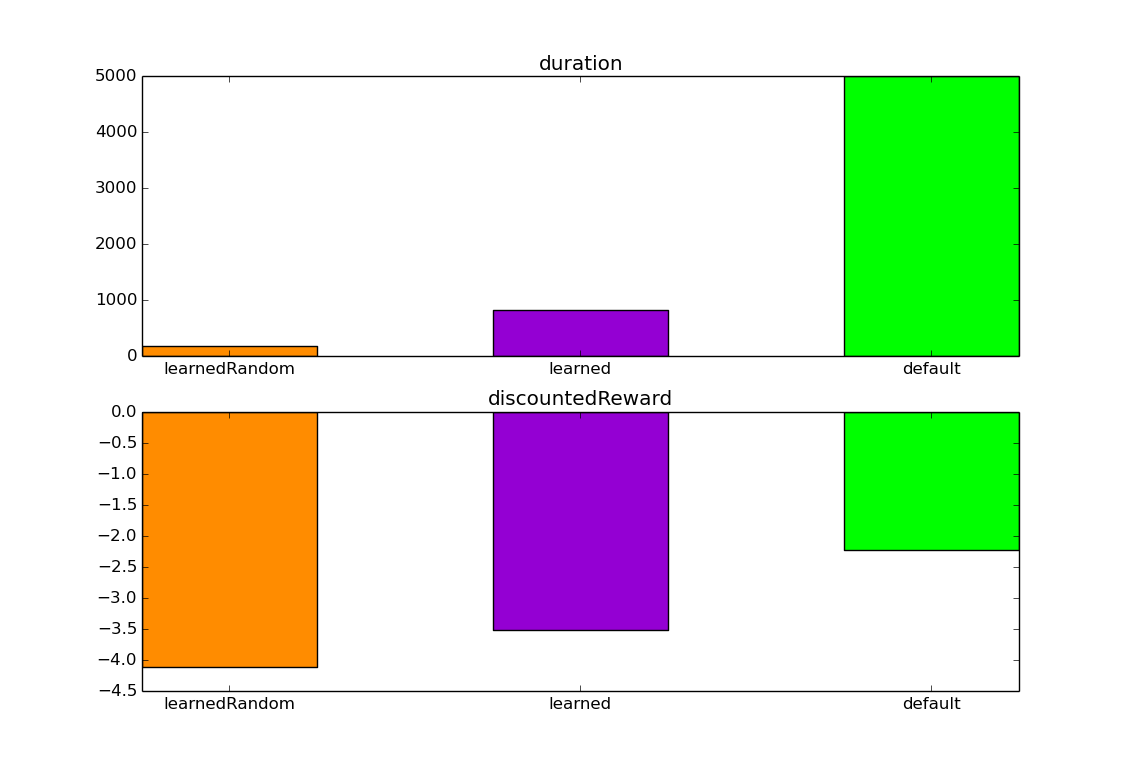
\includegraphics[scale=0.5]{figures/sarsaDiscrete_lam_0_7_6500_bar_all_controllers.png}
\caption{$\lambda = 0.7$}
\label{figures/sarsaDiscrete_lam_0_7_6500_bar_all_controllers.png}
\end{figure}

\begin{figure}
\centering
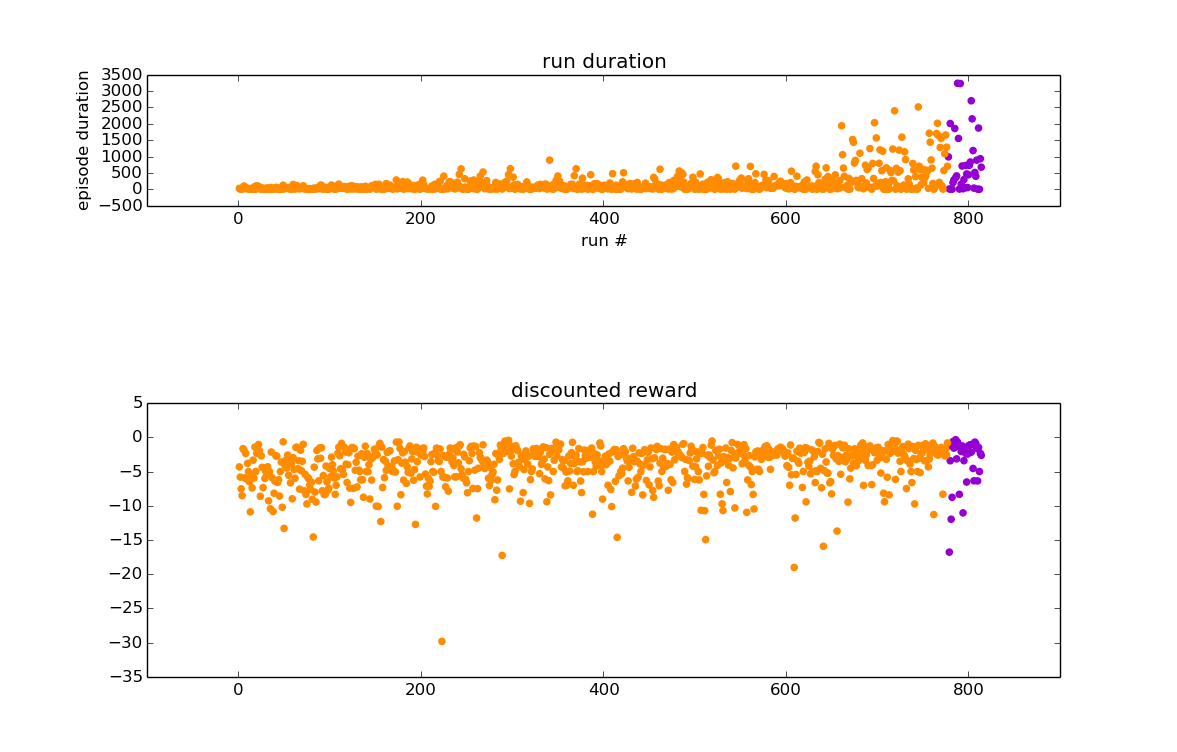
\includegraphics[scale=0.5]{figures/sarsaDiscrete_lam_0_7_6500_time_series_learned_controllers.png}
\caption{$\lambda = 0.7$}
\label{figures/sarsaDiscrete_lam_0_7_6500_time_series_learned_controllers.png}
\end{figure}


\begin{figure}
\centering
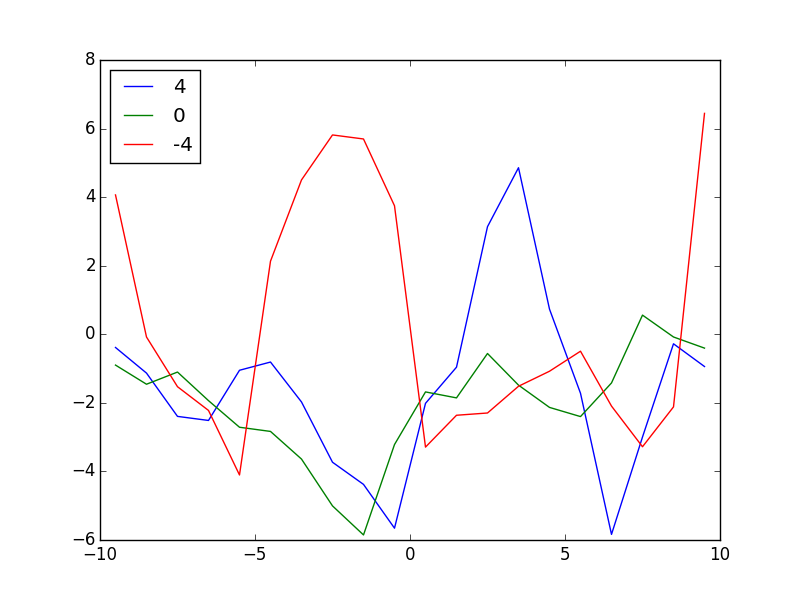
\includegraphics[scale=0.5]{figures/sarsa_cts_weights.png}
\caption{$\lambda = 0.7$}
\label{figures/sarsa_cts_weights.png}
\end{figure}



\begin{figure}
\centering
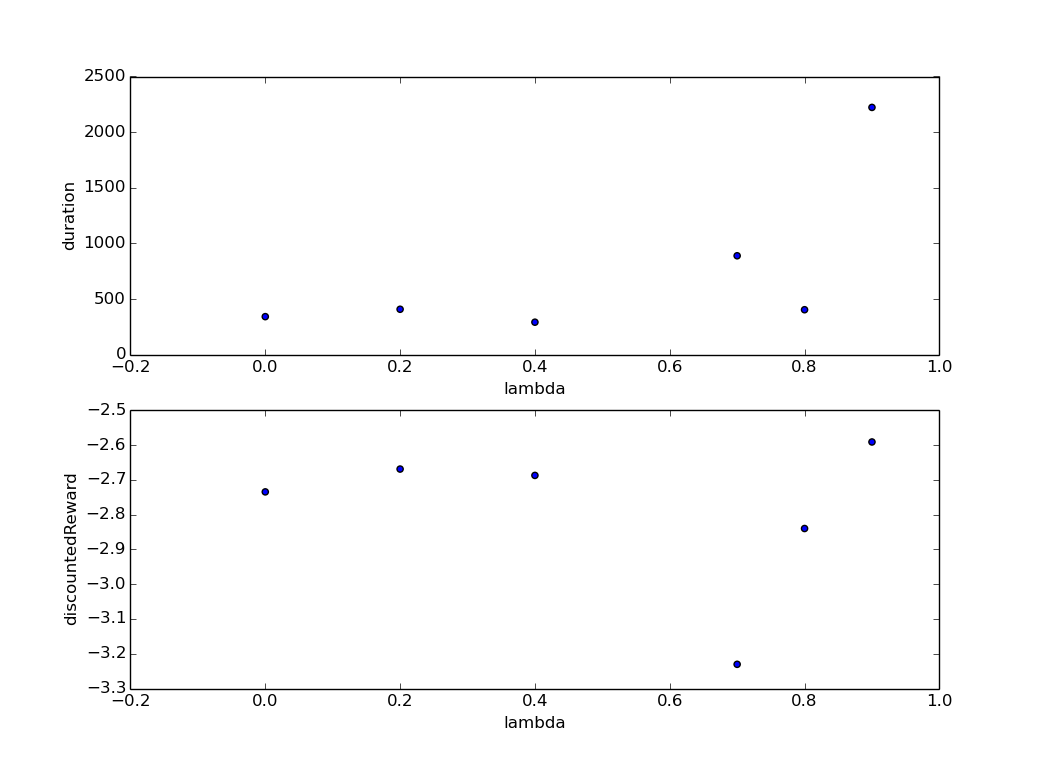
\includegraphics[scale=0.5]{figures/discreteSARSALamComparison.png}
\caption{$\lambda = 0.7$}
\label{figures/discreteSARSALamComparison.png}
\end{figure}

\begin{figure}
\centering
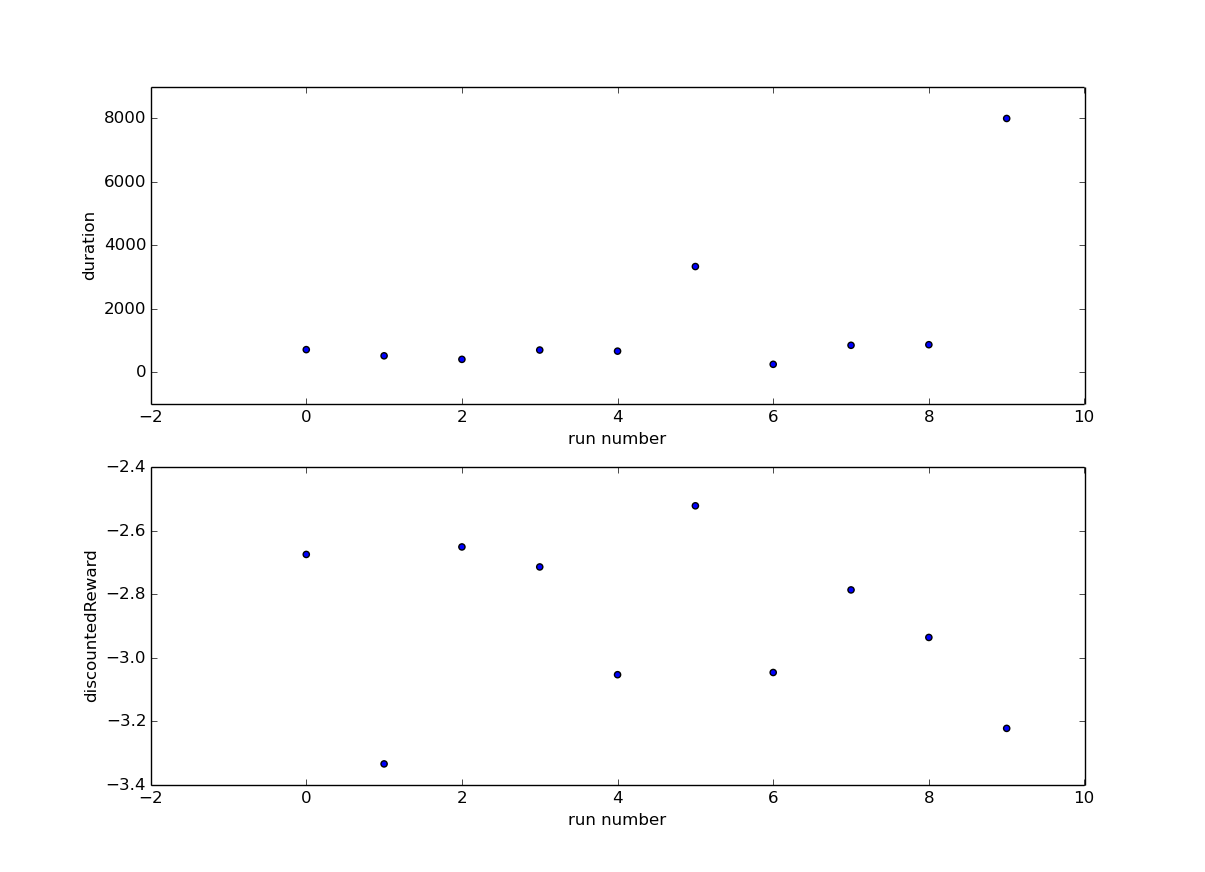
\includegraphics[scale=0.5]{figures/sarsaMultiple.png}
\caption{$\lambda = 0.7$}
\label{figures/sarsaMultiple.png}
\end{figure}


\begin{figure}
\centering
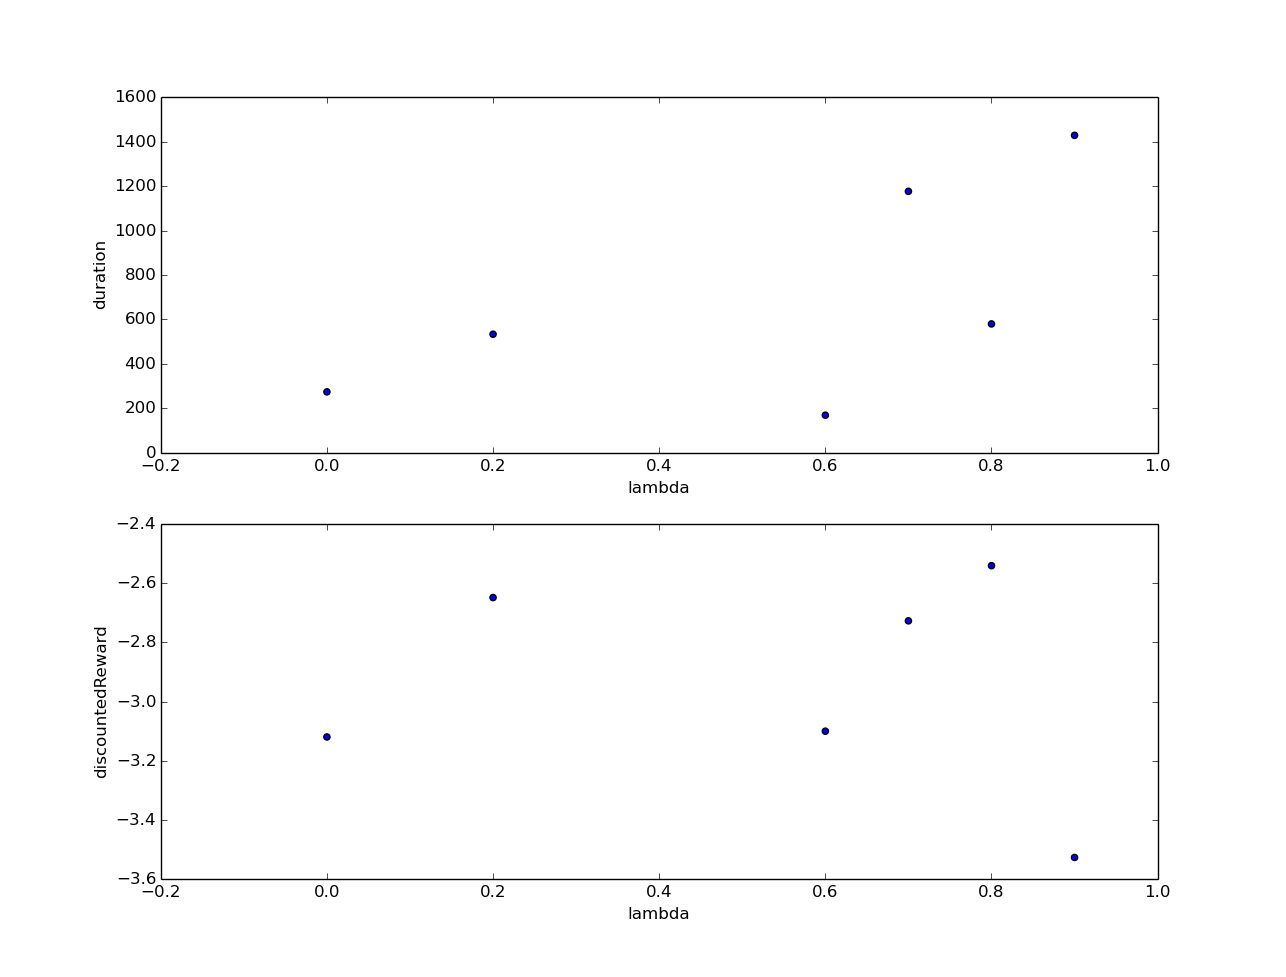
\includegraphics[scale=0.5]{figures/discreteQLearningLamComparison.png}
\caption{$\lambda = 0.7$}
\label{figures/discreteQLearningLamComparison.png}
\end{figure}



\begin{figure}
\centering
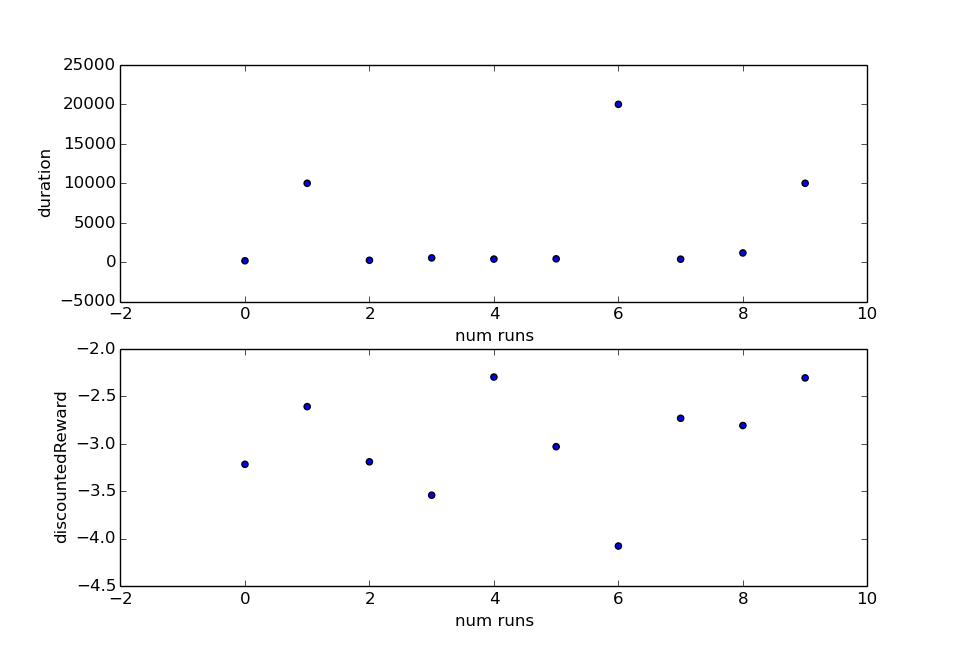
\includegraphics[scale=0.5]{figures/qlearningMultiple.png}
\caption{$\lambda = 0.7$}
\label{figures/qlearningMultiple.png}
\end{figure}


\begin{figure}
\centering
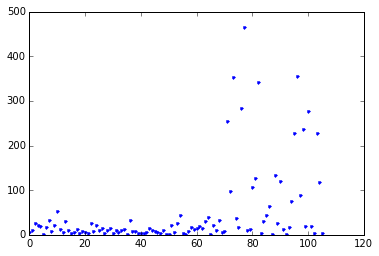
\includegraphics[scale=0.5]{figures/policySearch_zeroVector_duration.png}
\caption{Roll-out duration vs. roll-out trial number, for Episodic REINFORCE}
\label{figures/policySearch_zeroVector_duration.png}
\end{figure}


\begin{figure}
\centering
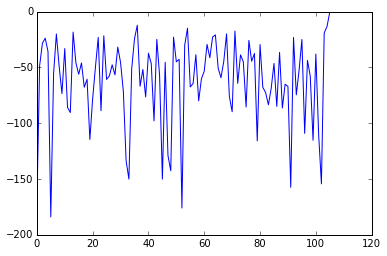
\includegraphics[scale=0.5]{figures/policySearch_zeroVector_discR.png}
\caption{Discounted reward vs. roll-out trial number, for Episodic REINFORCE}
\label{figures/policySearch_zeroVector_discR.png}
\end{figure}

\begin{figure}
\centering
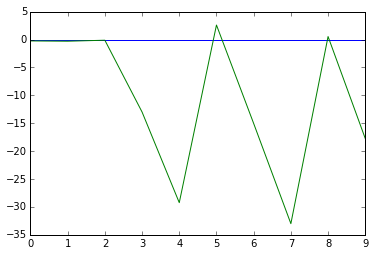
\includegraphics[scale=0.5]{figures/policySearch_zeroVector_weights.png}
\caption{Initial (zero-vector) and final weights, from Episodic REINFORCE after ~100 trials}
\label{figures/policySearch_zeroVector_weights.png}
\end{figure}





\bibliography{example_paper}
\bibliographystyle{icml2015}

\end{document} 


% This document was modified from the file originally made available by
% Pat Langley and Andrea Danyluk for ICML-2K. This version was
% created by Lise Getoor and Tobias Scheffer, it was slightly modified  
% from the 2010 version by Thorsten Joachims & Johannes Fuernkranz, 
% slightly modified from the 2009 version by Kiri Wagstaff and 
% Sam Roweis's 2008 version, which is slightly modified from 
% Prasad Tadepalli's 2007 version which is a lightly 
% changed version of the previous year's version by Andrew Moore, 
% which was in turn edited from those of Kristian Kersting and 
% Codrina Lauth. Alex Smola contributed to the algorithmic style files.  
